\documentclass[12pt,a4paper]{article}
% \documentclass[12pt,a4paper]{IEEEtran}

%\pdfoutput=1

\usepackage[utf8]{inputenc}
\usepackage[T1]{fontenc}
\usepackage[english]{babel}
\usepackage{amsmath}
\usepackage{mathabx}
\usepackage{lmodern}
\usepackage{units}
\usepackage{siunitx}
\usepackage{icomma}
\usepackage{graphicx}
\usepackage{caption}
\usepackage{subcaption}
\usepackage{courier}
\usepackage{color}
\usepackage{pgf}
\newcommand{\N}{\ensuremath{\mathbbm{N}}}
\newcommand{\Z}{\ensuremath{\mathbbm{Z}}}
\newcommand{\Q}{\ensuremath{\mathbbm{Q}}}
\newcommand{\R}{\ensuremath{\mathbbm{R}}}
\newcommand{\C}{\ensuremath{\mathbbm{C}}}
\newcommand{\rd}{\ensuremath{\mathrm{d}}}
\newcommand{\id}{\ensuremath{\,\rd}}
\usepackage{hyperref}
% \usepackage{a4wide} % puts the page numbering further down the page.
\usepackage{pdfpages}
\usepackage{epstopdf}
\DeclareGraphicsExtensions{.eps}

\title{Handin 3 MKM135}
\author{Marcus Malmquist}
\date{\today}

\begin{document}
\maketitle
\section{Task 1}
\begin{figure}[!ht]
  \centering
  \noindent\makebox[\textwidth]{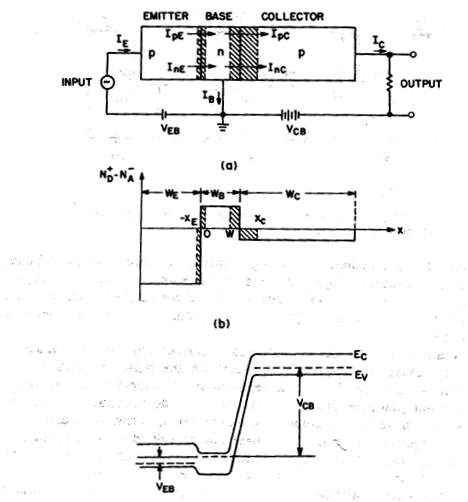
\includegraphics[width=0.7\textwidth]{image.png}}
  \caption{The figure depicts n-p-n BJT transistor with relevant variables used in the calculations.}
  \label{fig:schematic}
\end{figure}
When the transistor is active the hole current flowing into the base is the total base current and the electron current flowing into the emitter is the total emitter current.
This gives the equation to solve (\ref{eq:beta}).
\begin{equation}
  \label{eq:beta}
  \beta_{BnEp}=\frac{I_{B}}{I_{E}}
\end{equation}
From Kirchoff's current law we also have (\ref{eq:bjt}) for a BJT transistor.
\begin{equation}
  \label{eq:bjt}
  I_{E}=I_{B}+I_{C}
\end{equation}

The sought expression can then be reduced to (\ref{eq:expr}).
\begin{equation}
  \label{eq:expr}
  \beta_{BnEp}=1-\frac{I_{C}}{I_{E}}
\end{equation}
$I_C$ and $I_E$ can be seen in (\ref{eq:i_c}) and (\ref{eq:i_e}).
\begin{equation}
  \label{eq:i_c}
  \begin{array}{{rcl}}
    I_C & = & A[J_p(x=0) + J_n(x=-x_E)] \\
        & = & A\big [-qD_B\frac{\partial p}{\partial x}\big |_{x=0} - qD_E\frac{\partial n}{\partial x}\big |_{x=-x_E}\big ]
  \end{array}
\end{equation}
\begin{equation}
  \label{eq:i_e}
  \begin{array}{{rcl}}
    I_E & = & A[J_p(x=W) + J_n(x=x_C)] \\
        & = & A\big [-qD_B\frac{\partial p}{\partial x}\big |_{x=W} - qD_E\frac{\partial n}{\partial x}\big |_{x=x_C}\big ]
  \end{array}
\end{equation}
The hole and electron distribution in the emitter and collector are given by (\ref{eq:px}) and (\ref{eq:nx}).
\begin{equation}
  \label{eq:px}
  p(x) = p_B+\frac{p'(W)-p'(0)e^{-W/L_B}}{2\sinh(W/L_B)}e^{x/L_B} - \frac{p'(W)-p'(0)e^{W/L_B}}{2\sinh(W/L_B)}e^{-x/L_B}
\end{equation}
\begin{equation}
  \label{eq:nx}
  n(x) =
  \begin{cases}
    n_E+n'(-x_E)\exp\big(\frac{x+x_E}{L_E}\big) & x<x_E \\
    n_C+n'(x_C)\exp\big(-\frac{x-x_C}{L_E}\big)
  \end{cases}
\end{equation}
where $p'(W)$, $p'(0)$, $n'(-x_E)$ and $n'(x_C)$ can be seen in (\ref{eq:constants})
\begin{subequations}
  \label{eq:constants}
  \begin{align}
    p'(W) & = p_B\bigg[\exp\bigg(\frac{qV_{CB}}{kT}\bigg)-1\bigg]\\
    p'(0) & = p_B\bigg[\exp\bigg(\frac{qV_{EB}}{kT}\bigg)-1\bigg]\\
    n'(-x_E) & = n_E\bigg[\exp\bigg(\frac{qV_{EB}}{kT}\bigg)-1\bigg]\\
    n'(x_C) & = n_C\bigg[\exp\bigg(\frac{qV_{CB}}{kT}\bigg)-1\bigg]
  \end{align}
\end{subequations}
where $p_B$ is the equilibrium minority carrier density in the base,
$n_E$ is the equilibrium minority carrier density in the emitter,
$n_C$ is the equilibrium minority carrier density in the collector.

\section{Task 2}
\subsection{a}
The curoff frequency for the transistor is described by (\ref{eq:f_t})
\begin{equation}
  \label{eq:f_t}
  f_T=\frac{1}{2\pi \tau_{ec}}
\end{equation}
where $\tau_{ec}=\tau_{E}+\tau_{B}+\tau_{C}+\tau'_{C}$.\\
Emitter depletion-layer charging time $\tau_{E}=r_e(C_e+C_c+C_p)$. $r_e$ is the emitter resistance, $C_e$ is the emitter capacitance, $C_c$ is the collector capacitance and $C_p$ is any parasitic capacitance connected to the base.\\
\noindent Base-layer charging time $\tau_{B}=\frac{W^2}{2(1+(E_{bi}/E_{0})^{3/2}) D_B}$.\\
\noindent Collector depletion-layer charging time $\tau_C=\frac{x_C-W}{2v_s}$. $v_s$: saturation velocity.\\
\noindent Collector charging time: $\tau'_C=r_{c}C_c$ can be neglected.

(\ref{eq:f_t}) then becomes (\ref{eq:f_T})
\begin{equation}
  \label{eq:f_T}
  f_T=\bigg\{2\pi\bigg[r_e(C_e+C_c+C_p)+\frac{W^2}{2(1+(E_{bi}/E_{0})^{3/2}) D_B}+\frac{x_C-W}{2v_s}\bigg]\bigg\}^{-1}
\end{equation}
I was not able to find how these values relate to the design.
\end{document}